\section{Results}

Having established analytically the resource that tracks the sampling cost (Sec.~\ref{sec:resource}), we
now demonstrate the method and that resource numerically. We validate the reconstruction against exact
diagonalization, map the resource axis across lattices
and a nineteen-molecule chemical suite, benchmark the time-evolution selector against standard classical
selectors (conceding the strongest, heat-bath CI), and scale the demonstration toward the beyond-classical regime.

\subsection{Validation}
On Hubbard chains the bitstring-sampled subspace reproduces the exact multi-peak single-particle
spectral function (Fig.~\ref{fig:method}). The relative-$L_1$ error falls toward zero
as the time-evolution sampling discovers the spectral configurations, reaching $0.017$ for the
complete-subspace reconstruction (panel a; the $8$-seed finite-shot curve of panel b flattens toward
$\approx0.019$), and the addition-branch sum rule $\int A^{+}\,d\omega=1-\langle \hat n_p\rangle$ is satisfied
exactly---confirming that the classically-assembled Green's function of Eq.~\eqref{eq:green} inherits
the accuracy of the sampled subspace, not of any device-side estimation. The same primitive extends to
the momentum-dependent $A(k,\omega)$---whose dispersing lower and upper Hubbard bands and mid-gap Fermi
level are shown \emph{exactly} in Fig.~\ref{fig:lattice}---and to the dynamical structure factor
$S(q,\omega)$ from a number-conserving density seed (Fig.~\ref{fig:sqw}): a single sampling primitive
covers the photoemission and density-response channels that classically require separate dynamical-DMRG
computations~\cite{jeckelmann2002,nocera2016}. From a spin seed the same primitive furnishes the spin
structure factor $S^{zz}(q,\omega)$ (Fig.~\ref{fig:spin}), and the two collective responses lay bare
spin--charge separation in the two-particle channel: the charge continuum is \emph{gapped} by the Mott
gap $\Delta$, whereas the spin continuum is \emph{gapless} (in the thermodynamic limit), its bandwidth set by the far smaller exchange $J=4t^2/U$.
At subspace saturation the bitstring-sampled reconstruction
reproduces the exact result at every momentum to relative-$L_1$ below $\sim\!0.5\%$
(Fig.~\ref{fig:akwsampled}: the sampled $A(k,\omega)$ overlays the exact target across the Brillouin
zone, mean per-momentum error $2.2\times10^{-3}$, at a subspace of $85\%$ of the $(N{\pm}1)$ sector);
crucially, however---and unlike the ground-state
energy---saturating a \emph{full} dynamical spectral function requires a substantial---though
\emph{shrinking}---fraction of the $(N{+}1)$ sector ($0.92$ at $L=4$ down to $0.08$ at $L=14$,
Fig.~\ref{fig:scaling}), because the spectral weight
is distributed across the excited-state spectrum rather than concentrated in a few dominant
configurations. This subspace-fraction cost, not any device-side accuracy, is the resource that
Sec.~\ref{sec:resource} analyses. The continued-fraction reconstruction itself carries the standard
Lanczos caveats---finite sampling of the subspace and loss of orthogonality at high recursion order can
seed spurious low-weight poles---mitigated here by seed averaging and the finite broadening $\eta$.

\begin{figure}[htbp]\centering% native \input fragment (fig:method) — fonts = document body (11pt) exactly
\definecolor{inkPrim}{HTML}{1B1B1B}\definecolor{inkMute}{HTML}{6E6E6E}\definecolor{clExact}{HTML}{1F3A5F}
\definecolor{coral}{HTML}{F0653F}\definecolor{gridClr}{HTML}{ECEAE5}\definecolor{thm}{HTML}{2E7D5B}
\begin{tikzpicture}[font=\rmfamily]
\begin{groupplot}[
  group style={group size=2 by 1, horizontal sep=1.9cm},
  width=7.7cm, height=5.9cm, paperaxis,
  label style={font=\small}, tick label style={font=\footnotesize},
  axis line style={inkPrim, line width=0.6pt}, tick style={inkPrim, line width=0.6pt},
  title style={yshift=1pt},
]
% ---- (a) A(w): exact vs bitstring-sampled ----
\nextgroupplot[
  xlabel={frequency \; $\omega/t$}, ylabel={$A(\omega)$},
  title={(a)\quad reconstruction of $A(\omega)$ from $5.2\times10^{4}$ shots},
  xmin=3, xmax=14, ymin=0, ymax=0.50, ymajorgrids, y grid style={gridClr},
  legend style={draw=none, fill=white, fill opacity=0.75, text opacity=1, at={(0.985,0.985)}, anchor=north east}, legend cell align=left,
]
  \addplot[draw=none, fill=clExact, fill opacity=0.16, forget plot] table[x=w,y=Aex]{aw_method.dat} \closedcycle;
  \addplot[clExact, line width=1.3pt] table[x=w,y=Aex]{aw_method.dat}; \addlegendentry{exact}
  \addplot[coral, line width=1.1pt, dash pattern=on 3pt off 2.2pt] table[x=w,y=Asm]{aw_method.dat}; \addlegendentry{bitstring-sampled}
  \node[anchor=north east, align=right, inkPrim] at (rel axis cs:0.985,0.56)
     {rel-$L_1=0.017$\\[-1pt] $\int_W\! A_{\mathcal S}=0.4865$};
% ---- (b) convergence: the measured curve only.  The dashed 'geometric (Thm 1)' series
%      and the rho ~ 1.7 label are REMOVED: Sec. 4.2 withdraws that fit and its
%      attribution to the moment theorem. ----
\nextgroupplot[
  xlabel={Krylov order \; $K$ \; (time-evolution steps)}, ylabel={rel-$L_1$ error},
  title={(b)\quad error versus Krylov order},
  xmin=-0.4, xmax=12.4, ymode=log, ymin=0.013, ymax=2.6, ymajorgrids, y grid style={gridClr},
  ytick={0.02,0.05,0.1,0.2,0.5}, yticklabels={$2\%$,$5\%$,$10\%$,$20\%$,$50\%$},
  legend style={draw=none, fill=white, fill opacity=0.85, text opacity=1, at={(0.985,0.985)}, anchor=north east}, legend cell align=left,
]
  \fill[inkMute, fill opacity=0.06] (axis cs:-0.4,0.013) rectangle (axis cs:4,2.6);
  \node[inkPrim, anchor=center, align=center] at (axis cs:1.75,0.19) {discovery\\ regime};
  \addplot[name path=lo, draw=none, forget plot] coordinates {(0,0.5495) (1,0.5169) (2,0.5125) (3,0.5072) (4,0.3953) (5,0.1346) (6,0.0822) (7,0.0481) (8,0.0297) (9,0.0227) (10,0.0191) (11,0.0172) (12,0.0132)};
  \addplot[name path=hi, draw=none, forget plot] coordinates {(0,0.6261) (1,0.6267) (2,0.5807) (3,0.5948) (4,0.4793) (5,0.1820) (6,0.1081) (7,0.0713) (8,0.0402) (9,0.0307) (10,0.0275) (11,0.0259) (12,0.0239)};
  \addplot[coral, fill opacity=0.16, forget plot] fill between[of=lo and hi];
  \addplot[coral, line width=1.3pt, mark=*, mark size=2.2pt,
           mark options={fill=coral, draw=white, line width=0.4pt}] coordinates {(0,0.5878) (1,0.5718) (2,0.5466) (3,0.5510) (4,0.4373) (5,0.1583) (6,0.0951) (7,0.0597) (8,0.0350) (9,0.0267) (10,0.0233) (11,0.0216) (12,0.0185)}; \addlegendentry{sampled (8 seeds)}
\end{groupplot}
\end{tikzpicture}

\caption{\textbf{The method, validated---and its convergence matches the theorem.} \textbf{(a)}~The
bitstring-sampled single-particle spectral function reproduces the exact $A(\omega)$ (Hubbard $L=6$,
$U/t=8$; broadening $\eta=0.15\,t$) to relative-$L_1$ $0.017$---the exact (filled) and reconstructed
(dashed) curves are indistinguishable---and the reconstructed spectral weights obey the exact addition-branch sum
rule $\int A^{+}\,d\omega=0.500=1-\langle n_p\rangle$ to machine precision (the panel shows the addition branch $\omega>0$; the full $A$ integrates to $1$). \textbf{(b)}~Convergence of the relative-$L_1$ error with
the Krylov order $K$ (number of time-evolution steps sampled), seed-averaged over eight independent
runs (band $=$ standard deviation). Two regimes appear: a short \emph{discovery} phase in which the
time-evolution sampling first locates the spectral configurations, followed by a \emph{geometric
collapse} $\text{rel-}L_1\sim\rho^{-K}$ with $\rho\approx1.7$---precisely the geometric convergence
guaranteed by the moment-exactness theorem (Thm.~\ref{thm:b2}, App.~\ref{app:b2}). The sampled error
tracks the geometric law until it flattens toward the $8$-seed finite-shot value ($\approx0.019$ at $K=12$); the
complete-subspace reconstruction of panel (a) reaches $0.017$.}\label{fig:method}\end{figure}

\begin{figure}[htbp]\centering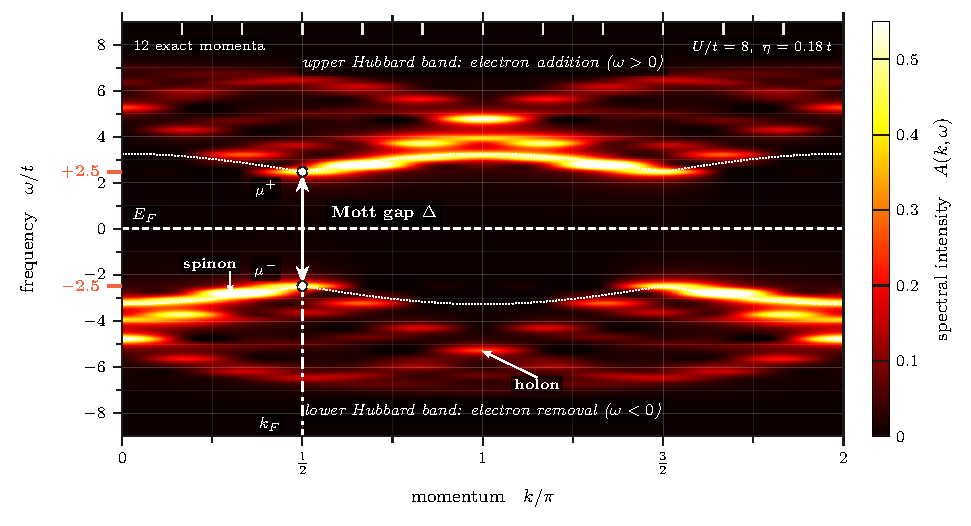
\includegraphics[width=\textwidth]{figs/fig_akw_native.pdf}
\caption{\textbf{Momentum-resolved spectral function: the exact dynamical target.} The
single-particle spectral function $A(k,\omega)$ of the half-filled Hubbard chain ($U/t=8$, $L=12$,
Lorentzian broadening $\eta=0.18\,t$), computed exactly from the resolvent $\langle\phi|(z-\hat H)^{-1}|\phi\rangle$ via the
Haydock continued fraction~\cite{haydock1972} over the full $(N{\pm}1)$ sectors (equivalent to the Lehmann sum in exact arithmetic)---the frequency- and momentum-resolved
observable that sample-based diagonalization targets but its energy-only output cannot itself deliver.
The two dispersing Hubbard bands---electron removal (lower, $\omega<0$; photoemission) and electron
addition (upper, $\omega>0$; inverse photoemission)---are separated by the correlation-driven
\emph{Mott gap} $\Delta=\mu^{+}-\mu^{-}=4.97\,t$ between the highest occupied state ($\mu^{-}$, lower
edge) and the lowest unoccupied state ($\mu^{+}$, upper edge), obtained from the exact $(N{\pm}1)$
ground-state energies (ticks at $\pm2.484\,t$); the broadened spectral peaks of the plotted $A(k_F,\omega)$
sit slightly wider, at $\pm2.49\,t$ (a $4.99\,t$ splitting), the $\sim\!0.02\,t$ excess being the
$\eta=0.18\,t$ Lorentzian broadening; the thermodynamic Lieb--Wu value~\cite{liebwu1968} is $4.68\,t$, the
$L=12$ excess being finite-size. The gap is \emph{direct} at the
Fermi momentum $k_F=\pi/2$. Particle--hole symmetry places the Fermi level at mid-gap ($\omega=0$),
verified to machine precision, and each momentum obeys the analytic spectral sum rule
$\int A(k,\omega)\,d\omega=1$ (the plotted broadened grid recovers it to $\sim\!2\%$ within the $\pm9t$ window).
The lower Hubbard band is not a single quasiparticle band but a \emph{spin--charge-separated} continuum:
a narrow spinon branch (bandwidth $\pi J/2=0.79\,t$~\cite{descloizeaux1962}, $J=4t^2/U$; dashed, validated against the exact
peak dispersion to ${<}0.1\,t$) rides a broad holon (charge, ${\sim}4t$) continuum---the hallmark
fractionalization of the 1D Mott insulator~\cite{liebwu1968}.
The momentum axis is a periodic cubic-spline interpolation of the $12$ physical momenta (ticks, top).
Faithfully \emph{sampling} this full momentum-resolved observable---as opposed to the ground-state
energy---requires a large fraction of the $(N{+}1)$ sector (Fig.~\ref{fig:scaling}), the cost
quantified in Sec.~\ref{sec:resource}.}\label{fig:lattice}\end{figure}

\begin{figure}[htbp]\centering% Sampled-vs-exact A(k,omega): REAL reconstruction (L=8 chain, U/t=8, 85% of the (N+-1) sector).
% Generated from sampled_akw_L8.json (mean per-k rel-L1 0.0022, max 0.0033); no hand-typed numbers.
\definecolor{akExact}{HTML}{1B1B1B}\definecolor{akSamp}{HTML}{D55E00}\definecolor{akInk}{HTML}{1B1B1B}
\begin{tikzpicture}
\begin{groupplot}[group style={group size=2 by 1, horizontal sep=1.7cm},
  width=8.2cm, height=6.2cm, paperaxis,
  title style={at={(0,1)},anchor=south west,font=\normalsize\bfseries,yshift=2pt},
  label style={font=\normalsize}, tick label style={font=\footnotesize}]
\nextgroupplot[title={(a)~sampled vs exact $A(k,\omega)$},
  xlabel={$\omega-E_0\ (t)$}, ylabel={$A(k,\omega)$ (offset by $k$)}, xmin=-9,xmax=9,
  ymin=-0.3,ymax=2.85, ytick=\empty, xtick={-8,-4,0,4,8},
  legend style={font=\footnotesize,at={(0.03,0.985)},anchor=north west,legend columns=1,draw=none,fill=white,fill opacity=0.55,text opacity=1},legend cell align=left]
\addplot[akExact,line width=1.2pt,fill=akExact,fill opacity=0.06] coordinates {(-9.000,0.0007) (-8.910,0.0007) (-8.820,0.0007) (-8.730,0.0007) (-8.639,0.0007) (-8.549,0.0008) (-8.459,0.0008) (-8.369,0.0008) (-8.279,0.0008) (-8.189,0.0008) (-8.098,0.0008) (-8.008,0.0008) (-7.918,0.0008) (-7.828,0.0009) (-7.738,0.0009) (-7.648,0.0009) (-7.558,0.0009) (-7.467,0.0009) (-7.377,0.0009) (-7.287,0.0010) (-7.197,0.0010) (-7.107,0.0010) (-7.017,0.0011) (-6.927,0.0011) (-6.836,0.0011) (-6.746,0.0011) (-6.656,0.0011) (-6.566,0.0011) (-6.476,0.0012) (-6.386,0.0012) (-6.295,0.0012) (-6.205,0.0013) (-6.115,0.0013) (-6.025,0.0014) (-5.935,0.0014) (-5.845,0.0015) (-5.755,0.0015) (-5.664,0.0016) (-5.574,0.0017) (-5.484,0.0017) (-5.394,0.0018) (-5.304,0.0018) (-5.214,0.0018) (-5.124,0.0019) (-5.033,0.0020) (-4.943,0.0020) (-4.853,0.0021) (-4.763,0.0022) (-4.673,0.0023) (-4.583,0.0024) (-4.492,0.0025) (-4.402,0.0026) (-4.312,0.0027) (-4.222,0.0028) (-4.132,0.0030) (-4.042,0.0031) (-3.952,0.0033) (-3.861,0.0034) (-3.771,0.0036) (-3.681,0.0038) (-3.591,0.0040) (-3.501,0.0043) (-3.411,0.0045) (-3.321,0.0048) (-3.230,0.0051) (-3.140,0.0055) (-3.050,0.0059) (-2.960,0.0064) (-2.870,0.0070) (-2.780,0.0077) (-2.689,0.0083) (-2.599,0.0087) (-2.509,0.0093) (-2.419,0.0100) (-2.329,0.0109) (-2.239,0.0119) (-2.149,0.0132) (-2.058,0.0147) (-1.968,0.0166) (-1.878,0.0188) (-1.788,0.0215) (-1.698,0.0250) (-1.608,0.0294) (-1.518,0.0349) (-1.427,0.0421) (-1.337,0.0520) (-1.247,0.0663) (-1.157,0.0874) (-1.067,0.1207) (-0.977,0.1760) (-0.886,0.2733) (-0.796,0.4437) (-0.706,0.6682) (-0.616,0.7105) (-0.526,0.5054) (-0.436,0.3171) (-0.346,0.2085) (-0.255,0.1500) (-0.165,0.1187) (-0.075,0.1032) (0.015,0.0988) (0.105,0.1041) (0.195,0.1208) (0.285,0.1546) (0.376,0.2183) (0.466,0.3365) (0.556,0.5306) (0.646,0.6887) (0.736,0.5799) (0.826,0.3703) (0.917,0.2297) (1.007,0.1506) (1.097,0.1050) (1.187,0.0771) (1.277,0.0591) (1.367,0.0468) (1.457,0.0380) (1.548,0.0316) (1.638,0.0267) (1.728,0.0229) (1.818,0.0199) (1.908,0.0175) (1.998,0.0155) (2.088,0.0139) (2.179,0.0125) (2.269,0.0113) (2.359,0.0103) (2.449,0.0094) (2.539,0.0087) (2.629,0.0080) (2.720,0.0074) (2.810,0.0069) (2.900,0.0065) (2.990,0.0060) (3.080,0.0057) (3.170,0.0053) (3.260,0.0050) (3.351,0.0048) (3.441,0.0045) (3.531,0.0043) (3.621,0.0041) (3.711,0.0039) (3.801,0.0037) (3.891,0.0036) (3.982,0.0034) (4.072,0.0033) (4.162,0.0032) (4.252,0.0031) (4.342,0.0030) (4.432,0.0029) (4.523,0.0028) (4.613,0.0027) (4.703,0.0027) (4.793,0.0026) (4.883,0.0025) (4.973,0.0025) (5.063,0.0024) (5.154,0.0024) (5.244,0.0023) (5.334,0.0023) (5.424,0.0023) (5.514,0.0023) (5.604,0.0022) (5.694,0.0022) (5.785,0.0022) (5.875,0.0022) (5.965,0.0022) (6.055,0.0022) (6.145,0.0023) (6.235,0.0023) (6.326,0.0023) (6.416,0.0023) (6.506,0.0024) (6.596,0.0025) (6.686,0.0025) (6.776,0.0026) (6.866,0.0027) (6.957,0.0029) (7.047,0.0030) (7.137,0.0033) (7.227,0.0036) (7.317,0.0041) (7.407,0.0048) (7.497,0.0052) (7.588,0.0050) (7.678,0.0049) (7.768,0.0049) (7.858,0.0052) (7.948,0.0056) (8.038,0.0062) (8.129,0.0070) (8.219,0.0080) (8.309,0.0092) (8.399,0.0105) (8.489,0.0120) (8.579,0.0141) (8.669,0.0171) (8.760,0.0213) (8.850,0.0274) (8.940,0.0367)} \closedcycle;
\addplot[akSamp,line width=1.1pt,dash pattern=on 4pt off 2.5pt] coordinates {(-9.000,0.0007) (-8.910,0.0007) (-8.820,0.0007) (-8.730,0.0007) (-8.639,0.0007) (-8.549,0.0008) (-8.459,0.0008) (-8.369,0.0008) (-8.279,0.0008) (-8.189,0.0008) (-8.098,0.0008) (-8.008,0.0008) (-7.918,0.0008) (-7.828,0.0008) (-7.738,0.0009) (-7.648,0.0009) (-7.558,0.0009) (-7.467,0.0009) (-7.377,0.0009) (-7.287,0.0010) (-7.197,0.0010) (-7.107,0.0010) (-7.017,0.0010) (-6.927,0.0011) (-6.836,0.0011) (-6.746,0.0011) (-6.656,0.0011) (-6.566,0.0011) (-6.476,0.0012) (-6.386,0.0012) (-6.295,0.0013) (-6.205,0.0013) (-6.115,0.0013) (-6.025,0.0014) (-5.935,0.0014) (-5.845,0.0015) (-5.755,0.0016) (-5.664,0.0017) (-5.574,0.0017) (-5.484,0.0017) (-5.394,0.0017) (-5.304,0.0018) (-5.214,0.0018) (-5.124,0.0019) (-5.033,0.0020) (-4.943,0.0020) (-4.853,0.0021) (-4.763,0.0022) (-4.673,0.0023) (-4.583,0.0024) (-4.492,0.0025) (-4.402,0.0026) (-4.312,0.0027) (-4.222,0.0028) (-4.132,0.0030) (-4.042,0.0031) (-3.952,0.0033) (-3.861,0.0034) (-3.771,0.0036) (-3.681,0.0038) (-3.591,0.0040) (-3.501,0.0043) (-3.411,0.0046) (-3.321,0.0048) (-3.230,0.0051) (-3.140,0.0055) (-3.050,0.0059) (-2.960,0.0064) (-2.870,0.0070) (-2.780,0.0077) (-2.689,0.0083) (-2.599,0.0087) (-2.509,0.0093) (-2.419,0.0100) (-2.329,0.0109) (-2.239,0.0119) (-2.149,0.0132) (-2.058,0.0147) (-1.968,0.0166) (-1.878,0.0188) (-1.788,0.0215) (-1.698,0.0250) (-1.608,0.0294) (-1.518,0.0349) (-1.427,0.0422) (-1.337,0.0521) (-1.247,0.0663) (-1.157,0.0875) (-1.067,0.1208) (-0.977,0.1763) (-0.886,0.2738) (-0.796,0.4445) (-0.706,0.6689) (-0.616,0.7102) (-0.526,0.5046) (-0.436,0.3167) (-0.346,0.2083) (-0.255,0.1498) (-0.165,0.1186) (-0.075,0.1032) (0.015,0.0988) (0.105,0.1041) (0.195,0.1208) (0.285,0.1547) (0.376,0.2184) (0.466,0.3366) (0.556,0.5308) (0.646,0.6886) (0.736,0.5795) (0.826,0.3699) (0.917,0.2295) (1.007,0.1505) (1.097,0.1049) (1.187,0.0771) (1.277,0.0590) (1.367,0.0467) (1.457,0.0380) (1.548,0.0316) (1.638,0.0267) (1.728,0.0229) (1.818,0.0199) (1.908,0.0175) (1.998,0.0155) (2.088,0.0139) (2.179,0.0125) (2.269,0.0113) (2.359,0.0103) (2.449,0.0094) (2.539,0.0087) (2.629,0.0080) (2.720,0.0074) (2.810,0.0069) (2.900,0.0064) (2.990,0.0060) (3.080,0.0057) (3.170,0.0053) (3.260,0.0050) (3.351,0.0048) (3.441,0.0045) (3.531,0.0043) (3.621,0.0041) (3.711,0.0039) (3.801,0.0037) (3.891,0.0036) (3.982,0.0034) (4.072,0.0033) (4.162,0.0032) (4.252,0.0031) (4.342,0.0030) (4.432,0.0029) (4.523,0.0028) (4.613,0.0027) (4.703,0.0027) (4.793,0.0026) (4.883,0.0025) (4.973,0.0025) (5.063,0.0024) (5.154,0.0024) (5.244,0.0023) (5.334,0.0023) (5.424,0.0023) (5.514,0.0023) (5.604,0.0022) (5.694,0.0022) (5.785,0.0022) (5.875,0.0022) (5.965,0.0022) (6.055,0.0022) (6.145,0.0023) (6.235,0.0023) (6.326,0.0023) (6.416,0.0023) (6.506,0.0024) (6.596,0.0025) (6.686,0.0025) (6.776,0.0026) (6.866,0.0027) (6.957,0.0029) (7.047,0.0030) (7.137,0.0033) (7.227,0.0036) (7.317,0.0041) (7.407,0.0048) (7.497,0.0052) (7.588,0.0050) (7.678,0.0049) (7.768,0.0049) (7.858,0.0052) (7.948,0.0056) (8.038,0.0062) (8.129,0.0070) (8.219,0.0080) (8.309,0.0092) (8.399,0.0105) (8.489,0.0120) (8.579,0.0141) (8.669,0.0171) (8.760,0.0213) (8.850,0.0274) (8.940,0.0366)};
\addlegendentry{exact}\addlegendentry{sampled ($85\%$ sector)}
\node[akInk,font=\footnotesize,anchor=west] at (axis cs:5.2,0.424) {$k{=}0$};
\addplot[akExact,line width=1.2pt,fill=akExact,fill opacity=0.06] coordinates {(-9.000,0.7711) (-8.910,0.7711) (-8.820,0.7711) (-8.730,0.7711) (-8.639,0.7711) (-8.549,0.7712) (-8.459,0.7712) (-8.369,0.7712) (-8.279,0.7712) (-8.189,0.7712) (-8.098,0.7712) (-8.008,0.7712) (-7.918,0.7712) (-7.828,0.7713) (-7.738,0.7713) (-7.648,0.7713) (-7.558,0.7713) (-7.467,0.7713) (-7.377,0.7713) (-7.287,0.7713) (-7.197,0.7714) (-7.107,0.7714) (-7.017,0.7715) (-6.927,0.7715) (-6.836,0.7715) (-6.746,0.7715) (-6.656,0.7715) (-6.566,0.7715) (-6.476,0.7715) (-6.386,0.7715) (-6.295,0.7716) (-6.205,0.7716) (-6.115,0.7717) (-6.025,0.7717) (-5.935,0.7717) (-5.845,0.7718) (-5.755,0.7718) (-5.664,0.7718) (-5.574,0.7719) (-5.484,0.7719) (-5.394,0.7720) (-5.304,0.7721) (-5.214,0.7721) (-5.124,0.7722) (-5.033,0.7723) (-4.943,0.7724) (-4.853,0.7725) (-4.763,0.7726) (-4.673,0.7727) (-4.583,0.7728) (-4.492,0.7730) (-4.402,0.7731) (-4.312,0.7733) (-4.222,0.7735) (-4.132,0.7737) (-4.042,0.7740) (-3.952,0.7743) (-3.861,0.7747) (-3.771,0.7751) (-3.681,0.7757) (-3.591,0.7763) (-3.501,0.7771) (-3.411,0.7781) (-3.321,0.7794) (-3.230,0.7811) (-3.140,0.7834) (-3.050,0.7868) (-2.960,0.7917) (-2.870,0.7993) (-2.780,0.8121) (-2.689,0.8345) (-2.599,0.8727) (-2.509,0.9172) (-2.419,0.9200) (-2.329,0.8916) (-2.239,0.8742) (-2.149,0.8538) (-2.058,0.8277) (-1.968,0.8094) (-1.878,0.7988) (-1.788,0.7926) (-1.698,0.7888) (-1.608,0.7865) (-1.518,0.7852) (-1.427,0.7847) (-1.337,0.7849) (-1.247,0.7857) (-1.157,0.7874) (-1.067,0.7903) (-0.977,0.7951) (-0.886,0.8034) (-0.796,0.8182) (-0.706,0.8444) (-0.616,0.8813) (-0.526,0.8939) (-0.436,0.8628) (-0.346,0.8307) (-0.255,0.8120) (-0.165,0.8021) (-0.075,0.7972) (0.015,0.7953) (0.105,0.7946) (0.195,0.7937) (0.285,0.7934) (0.376,0.7943) (0.466,0.7965) (0.556,0.8000) (0.646,0.8052) (0.736,0.8129) (0.826,0.8243) (0.917,0.8418) (1.007,0.8700) (1.097,0.9178) (1.187,1.0031) (1.277,1.1501) (1.367,1.3198) (1.457,1.3048) (1.548,1.1292) (1.638,0.9898) (1.728,0.9100) (1.818,0.8649) (1.908,0.8381) (1.998,0.8212) (2.088,0.8100) (2.179,0.8021) (2.269,0.7965) (2.359,0.7924) (2.449,0.7892) (2.539,0.7867) (2.629,0.7848) (2.720,0.7832) (2.810,0.7820) (2.900,0.7809) (2.990,0.7801) (3.080,0.7794) (3.170,0.7788) (3.260,0.7783) (3.351,0.7779) (3.441,0.7776) (3.531,0.7773) (3.621,0.7771) (3.711,0.7770) (3.801,0.7769) (3.891,0.7768) (3.982,0.7768) (4.072,0.7768) (4.162,0.7768) (4.252,0.7769) (4.342,0.7771) (4.432,0.7772) (4.523,0.7775) (4.613,0.7778) (4.703,0.7782) (4.793,0.7786) (4.883,0.7791) (4.973,0.7798) (5.063,0.7806) (5.154,0.7815) (5.244,0.7827) (5.334,0.7841) (5.424,0.7859) (5.514,0.7881) (5.604,0.7910) (5.694,0.7947) (5.785,0.7996) (5.875,0.8065) (5.965,0.8161) (6.055,0.8304) (6.145,0.8524) (6.235,0.8886) (6.326,0.9516) (6.416,1.0640) (6.506,1.2376) (6.596,1.3463) (6.686,1.2253) (6.776,1.0546) (6.866,0.9466) (6.957,0.8863) (7.047,0.8516) (7.137,0.8305) (7.227,0.8170) (7.317,0.8080) (7.407,0.8019) (7.497,0.7977) (7.588,0.7951) (7.678,0.7937) (7.768,0.7935) (7.858,0.7942) (7.948,0.7950) (8.038,0.7962) (8.129,0.7997) (8.219,0.8071) (8.309,0.8216) (8.399,0.8481) (8.489,0.8842) (8.579,0.8924) (8.669,0.8590) (8.760,0.8272) (8.850,0.8084) (8.940,0.7980)} \closedcycle;
\addplot[akSamp,line width=1.1pt,dash pattern=on 4pt off 2.5pt] coordinates {(-9.000,0.7711) (-8.910,0.7711) (-8.820,0.7711) (-8.730,0.7711) (-8.639,0.7711) (-8.549,0.7712) (-8.459,0.7712) (-8.369,0.7712) (-8.279,0.7712) (-8.189,0.7712) (-8.098,0.7712) (-8.008,0.7712) (-7.918,0.7713) (-7.828,0.7713) (-7.738,0.7713) (-7.648,0.7713) (-7.558,0.7713) (-7.467,0.7713) (-7.377,0.7713) (-7.287,0.7714) (-7.197,0.7714) (-7.107,0.7714) (-7.017,0.7715) (-6.927,0.7714) (-6.836,0.7714) (-6.746,0.7715) (-6.656,0.7715) (-6.566,0.7715) (-6.476,0.7715) (-6.386,0.7715) (-6.295,0.7716) (-6.205,0.7716) (-6.115,0.7716) (-6.025,0.7717) (-5.935,0.7717) (-5.845,0.7717) (-5.755,0.7718) (-5.664,0.7718) (-5.574,0.7719) (-5.484,0.7719) (-5.394,0.7720) (-5.304,0.7721) (-5.214,0.7721) (-5.124,0.7722) (-5.033,0.7723) (-4.943,0.7724) (-4.853,0.7725) (-4.763,0.7726) (-4.673,0.7727) (-4.583,0.7728) (-4.492,0.7730) (-4.402,0.7731) (-4.312,0.7733) (-4.222,0.7735) (-4.132,0.7737) (-4.042,0.7740) (-3.952,0.7743) (-3.861,0.7747) (-3.771,0.7751) (-3.681,0.7757) (-3.591,0.7763) (-3.501,0.7771) (-3.411,0.7781) (-3.321,0.7794) (-3.230,0.7811) (-3.140,0.7835) (-3.050,0.7868) (-2.960,0.7918) (-2.870,0.7995) (-2.780,0.8123) (-2.689,0.8349) (-2.599,0.8733) (-2.509,0.9176) (-2.419,0.9196) (-2.329,0.8912) (-2.239,0.8741) (-2.149,0.8536) (-2.058,0.8275) (-1.968,0.8093) (-1.878,0.7987) (-1.788,0.7926) (-1.698,0.7888) (-1.608,0.7865) (-1.518,0.7852) (-1.427,0.7847) (-1.337,0.7849) (-1.247,0.7857) (-1.157,0.7874) (-1.067,0.7903) (-0.977,0.7952) (-0.886,0.8036) (-0.796,0.8184) (-0.706,0.8448) (-0.616,0.8816) (-0.526,0.8937) (-0.436,0.8623) (-0.346,0.8304) (-0.255,0.8118) (-0.165,0.8020) (-0.075,0.7972) (0.015,0.7953) (0.105,0.7945) (0.195,0.7937) (0.285,0.7934) (0.376,0.7943) (0.466,0.7965) (0.556,0.8000) (0.646,0.8053) (0.736,0.8130) (0.826,0.8245) (0.917,0.8420) (1.007,0.8703) (1.097,0.9184) (1.187,1.0042) (1.277,1.1519) (1.367,1.3209) (1.457,1.3034) (1.548,1.1275) (1.638,0.9888) (1.728,0.9094) (1.818,0.8646) (1.908,0.8379) (1.998,0.8211) (2.088,0.8099) (2.179,0.8021) (2.269,0.7965) (2.359,0.7923) (2.449,0.7892) (2.539,0.7867) (2.629,0.7848) (2.720,0.7832) (2.810,0.7820) (2.900,0.7809) (2.990,0.7801) (3.080,0.7794) (3.170,0.7788) (3.260,0.7783) (3.351,0.7779) (3.441,0.7776) (3.531,0.7773) (3.621,0.7771) (3.711,0.7770) (3.801,0.7769) (3.891,0.7768) (3.982,0.7768) (4.072,0.7768) (4.162,0.7768) (4.252,0.7769) (4.342,0.7771) (4.432,0.7772) (4.523,0.7775) (4.613,0.7778) (4.703,0.7781) (4.793,0.7786) (4.883,0.7791) (4.973,0.7798) (5.063,0.7806) (5.154,0.7815) (5.244,0.7827) (5.334,0.7841) (5.424,0.7859) (5.514,0.7881) (5.604,0.7909) (5.694,0.7946) (5.785,0.7996) (5.875,0.8064) (5.965,0.8160) (6.055,0.8302) (6.145,0.8521) (6.235,0.8882) (6.326,0.9507) (6.416,1.0625) (6.506,1.2358) (6.596,1.3464) (6.686,1.2271) (6.776,1.0560) (6.866,0.9474) (6.957,0.8868) (7.047,0.8519) (7.137,0.8307) (7.227,0.8171) (7.317,0.8081) (7.407,0.8019) (7.497,0.7978) (7.588,0.7951) (7.678,0.7937) (7.768,0.7935) (7.858,0.7942) (7.948,0.7950) (8.038,0.7961) (8.129,0.7996) (8.219,0.8070) (8.309,0.8214) (8.399,0.8477) (8.489,0.8838) (8.579,0.8926) (8.669,0.8595) (8.760,0.8275) (8.850,0.8086) (8.940,0.7981)};
\node[akInk,font=\footnotesize,anchor=west] at (axis cs:5.2,1.194) {$k{=}\pi/2$};
\addplot[akExact,line width=1.2pt,fill=akExact,fill opacity=0.06] coordinates {(-9.000,1.5416) (-8.910,1.5416) (-8.820,1.5416) (-8.730,1.5416) (-8.639,1.5416) (-8.549,1.5416) (-8.459,1.5416) (-8.369,1.5416) (-8.279,1.5416) (-8.189,1.5417) (-8.098,1.5417) (-8.008,1.5417) (-7.918,1.5417) (-7.828,1.5417) (-7.738,1.5417) (-7.648,1.5418) (-7.558,1.5418) (-7.467,1.5418) (-7.377,1.5418) (-7.287,1.5418) (-7.197,1.5418) (-7.107,1.5418) (-7.017,1.5419) (-6.927,1.5420) (-6.836,1.5420) (-6.746,1.5420) (-6.656,1.5419) (-6.566,1.5419) (-6.476,1.5419) (-6.386,1.5420) (-6.295,1.5420) (-6.205,1.5420) (-6.115,1.5420) (-6.025,1.5421) (-5.935,1.5421) (-5.845,1.5421) (-5.755,1.5422) (-5.664,1.5422) (-5.574,1.5423) (-5.484,1.5423) (-5.394,1.5424) (-5.304,1.5424) (-5.214,1.5425) (-5.124,1.5425) (-5.033,1.5426) (-4.943,1.5427) (-4.853,1.5428) (-4.763,1.5429) (-4.673,1.5430) (-4.583,1.5431) (-4.492,1.5433) (-4.402,1.5435) (-4.312,1.5436) (-4.222,1.5439) (-4.132,1.5441) (-4.042,1.5444) (-3.952,1.5448) (-3.861,1.5452) (-3.771,1.5458) (-3.681,1.5465) (-3.591,1.5474) (-3.501,1.5487) (-3.411,1.5505) (-3.321,1.5532) (-3.230,1.5574) (-3.140,1.5645) (-3.050,1.5771) (-2.960,1.5974) (-2.870,1.6151) (-2.780,1.6059) (-2.689,1.5852) (-2.599,1.5715) (-2.509,1.5644) (-2.419,1.5612) (-2.329,1.5602) (-2.239,1.5610) (-2.149,1.5632) (-2.058,1.5673) (-1.968,1.5739) (-1.878,1.5846) (-1.788,1.6026) (-1.698,1.6342) (-1.608,1.6910) (-1.518,1.7796) (-1.427,1.8381) (-1.337,1.7782) (-1.247,1.6896) (-1.157,1.6329) (-1.067,1.6013) (-0.977,1.5830) (-0.886,1.5719) (-0.796,1.5647) (-0.706,1.5598) (-0.616,1.5563) (-0.526,1.5539) (-0.436,1.5522) (-0.346,1.5509) (-0.255,1.5496) (-0.165,1.5485) (-0.075,1.5476) (0.015,1.5470) (0.105,1.5465) (0.195,1.5462) (0.285,1.5460) (0.376,1.5461) (0.466,1.5463) (0.556,1.5462) (0.646,1.5455) (0.736,1.5449) (0.826,1.5445) (0.917,1.5443) (1.007,1.5441) (1.097,1.5439) (1.187,1.5438) (1.277,1.5437) (1.367,1.5436) (1.457,1.5436) (1.548,1.5435) (1.638,1.5435) (1.728,1.5434) (1.818,1.5434) (1.908,1.5434) (1.998,1.5434) (2.088,1.5434) (2.179,1.5434) (2.269,1.5434) (2.359,1.5434) (2.449,1.5434) (2.539,1.5434) (2.629,1.5434) (2.720,1.5435) (2.810,1.5435) (2.900,1.5436) (2.990,1.5436) (3.080,1.5436) (3.170,1.5437) (3.260,1.5438) (3.351,1.5438) (3.441,1.5439) (3.531,1.5440) (3.621,1.5441) (3.711,1.5442) (3.801,1.5443) (3.891,1.5444) (3.982,1.5445) (4.072,1.5447) (4.162,1.5448) (4.252,1.5450) (4.342,1.5452) (4.432,1.5454) (4.523,1.5456) (4.613,1.5458) (4.703,1.5461) (4.793,1.5464) (4.883,1.5467) (4.973,1.5470) (5.063,1.5474) (5.154,1.5479) (5.244,1.5484) (5.334,1.5489) (5.424,1.5495) (5.514,1.5502) (5.604,1.5511) (5.694,1.5520) (5.785,1.5531) (5.875,1.5544) (5.965,1.5559) (6.055,1.5578) (6.145,1.5600) (6.235,1.5628) (6.326,1.5662) (6.416,1.5706) (6.506,1.5763) (6.596,1.5840) (6.686,1.5947) (6.776,1.6100) (6.866,1.6332) (6.957,1.6702) (7.047,1.7331) (7.137,1.8447) (7.227,2.0317) (7.317,2.2182) (7.407,2.1565) (7.497,1.9483) (7.588,1.7992) (7.678,1.7170) (7.768,1.6732) (7.858,1.6504) (7.948,1.6409) (8.038,1.6414) (8.129,1.6520) (8.219,1.6759) (8.309,1.7214) (8.399,1.8059) (8.489,1.9596) (8.579,2.1812) (8.669,2.2662) (8.760,2.0772) (8.850,1.8733) (8.940,1.7501)} \closedcycle;
\addplot[akSamp,line width=1.1pt,dash pattern=on 4pt off 2.5pt] coordinates {(-9.000,1.5416) (-8.910,1.5416) (-8.820,1.5416) (-8.730,1.5416) (-8.639,1.5416) (-8.549,1.5416) (-8.459,1.5416) (-8.369,1.5416) (-8.279,1.5417) (-8.189,1.5417) (-8.098,1.5417) (-8.008,1.5417) (-7.918,1.5417) (-7.828,1.5417) (-7.738,1.5418) (-7.648,1.5418) (-7.558,1.5417) (-7.467,1.5418) (-7.377,1.5418) (-7.287,1.5418) (-7.197,1.5418) (-7.107,1.5419) (-7.017,1.5419) (-6.927,1.5420) (-6.836,1.5420) (-6.746,1.5419) (-6.656,1.5419) (-6.566,1.5419) (-6.476,1.5419) (-6.386,1.5420) (-6.295,1.5420) (-6.205,1.5420) (-6.115,1.5420) (-6.025,1.5421) (-5.935,1.5421) (-5.845,1.5421) (-5.755,1.5422) (-5.664,1.5422) (-5.574,1.5423) (-5.484,1.5423) (-5.394,1.5424) (-5.304,1.5424) (-5.214,1.5425) (-5.124,1.5425) (-5.033,1.5426) (-4.943,1.5427) (-4.853,1.5428) (-4.763,1.5429) (-4.673,1.5430) (-4.583,1.5431) (-4.492,1.5433) (-4.402,1.5435) (-4.312,1.5436) (-4.222,1.5439) (-4.132,1.5441) (-4.042,1.5444) (-3.952,1.5448) (-3.861,1.5452) (-3.771,1.5458) (-3.681,1.5465) (-3.591,1.5475) (-3.501,1.5487) (-3.411,1.5505) (-3.321,1.5532) (-3.230,1.5575) (-3.140,1.5646) (-3.050,1.5773) (-2.960,1.5977) (-2.870,1.6152) (-2.780,1.6057) (-2.689,1.5850) (-2.599,1.5714) (-2.509,1.5643) (-2.419,1.5612) (-2.329,1.5602) (-2.239,1.5610) (-2.149,1.5632) (-2.058,1.5673) (-1.968,1.5739) (-1.878,1.5847) (-1.788,1.6028) (-1.698,1.6345) (-1.608,1.6914) (-1.518,1.7801) (-1.427,1.8381) (-1.337,1.7777) (-1.247,1.6892) (-1.157,1.6327) (-1.067,1.6011) (-0.977,1.5829) (-0.886,1.5718) (-0.796,1.5646) (-0.706,1.5597) (-0.616,1.5563) (-0.526,1.5539) (-0.436,1.5522) (-0.346,1.5509) (-0.255,1.5496) (-0.165,1.5485) (-0.075,1.5476) (0.015,1.5470) (0.105,1.5465) (0.195,1.5462) (0.285,1.5460) (0.376,1.5461) (0.466,1.5463) (0.556,1.5462) (0.646,1.5455) (0.736,1.5449) (0.826,1.5445) (0.917,1.5443) (1.007,1.5441) (1.097,1.5439) (1.187,1.5438) (1.277,1.5437) (1.367,1.5436) (1.457,1.5436) (1.548,1.5435) (1.638,1.5435) (1.728,1.5434) (1.818,1.5434) (1.908,1.5434) (1.998,1.5434) (2.088,1.5434) (2.179,1.5434) (2.269,1.5434) (2.359,1.5434) (2.449,1.5434) (2.539,1.5434) (2.629,1.5434) (2.720,1.5435) (2.810,1.5435) (2.900,1.5435) (2.990,1.5436) (3.080,1.5436) (3.170,1.5437) (3.260,1.5438) (3.351,1.5438) (3.441,1.5439) (3.531,1.5440) (3.621,1.5441) (3.711,1.5442) (3.801,1.5443) (3.891,1.5444) (3.982,1.5445) (4.072,1.5447) (4.162,1.5448) (4.252,1.5450) (4.342,1.5452) (4.432,1.5454) (4.523,1.5456) (4.613,1.5458) (4.703,1.5461) (4.793,1.5464) (4.883,1.5467) (4.973,1.5470) (5.063,1.5474) (5.154,1.5479) (5.244,1.5483) (5.334,1.5489) (5.424,1.5495) (5.514,1.5502) (5.604,1.5511) (5.694,1.5520) (5.785,1.5531) (5.875,1.5544) (5.965,1.5559) (6.055,1.5578) (6.145,1.5600) (6.235,1.5628) (6.326,1.5662) (6.416,1.5706) (6.506,1.5763) (6.596,1.5840) (6.686,1.5946) (6.776,1.6100) (6.866,1.6331) (6.957,1.6701) (7.047,1.7329) (7.137,1.8444) (7.227,2.0313) (7.317,2.2179) (7.407,2.1567) (7.497,1.9485) (7.588,1.7993) (7.678,1.7171) (7.768,1.6732) (7.858,1.6504) (7.948,1.6409) (8.038,1.6413) (8.129,1.6519) (8.219,1.6758) (8.309,1.7212) (8.399,1.8055) (8.489,1.9589) (8.579,2.1806) (8.669,2.2666) (8.760,2.0781) (8.850,1.8739) (8.940,1.7504)};
\node[akInk,font=\footnotesize,anchor=west] at (axis cs:5.2,1.965) {$k{=}\pi$};
\nextgroupplot[title={(b)~per-momentum error},
  xlabel={$k/\pi$}, ylabel={relative-$L_1$}, xmin=-0.1,xmax=2.0,
  ymin=0,ymax=0.006, xtick={0,0.5,1,1.5}, ytick={0,0.002,0.004},
  yticklabel style={/pgf/number format/fixed,/pgf/number format/precision=3}, ymajorgrids, grid style={draw=black!10}]
\addplot[akSamp,only marks,mark=*,mark size=2.6pt,mark options={fill=akSamp,draw=white,line width=0.6pt}] coordinates {(0.000,0.0009) (0.250,0.0023) (0.500,0.0033) (0.750,0.0022) (1.000,0.0011) (1.250,0.0022) (1.500,0.0033) (1.750,0.0023)};
\addplot[akExact,densely dotted,line width=0.8pt,domain=-0.1:2.0] {0.005};
\node[akInk,font=\footnotesize,anchor=north east] at (axis cs:1.95,0.0059) {$<0.5\%$ at every $k$};
\node[akInk,font=\footnotesize,anchor=south] at (axis cs:0.9,0.0038) {mean 2.2$\times10^{-3}$};
\end{groupplot}
\end{tikzpicture}

\caption{\textbf{The momentum-resolved spectral function reconstructed from bitstring-sampled subspaces,
overlaid on the exact target.} \textbf{(a)}~Bitstring-sampled $A(k,\omega)$ (dashed) versus the exact
Haydock result (solid, shaded) at three representative momenta ($k=0,\pi/2,\pi$; Hubbard chain, $L=8$,
$U/t=8$, $\eta=0.18\,t$; curves offset vertically by $k$), reconstructed by time-evolution
configuration sampling in the $(N{\pm}1)$ sectors and the classical Lehmann assembly of
Eq.~\eqref{eq:green}---not the exact target of Fig.~\ref{fig:lattice}, but the \emph{sampled} output.
\textbf{(b)}~Relative-$L_1$ error of the sampled reconstruction at every physical momentum, at a subspace
of $85\%$ of the $(N{\pm}1)$ sector: below $0.5\%$ throughout (mean $2.2\times10^{-3}$). The reconstruction
is faithful across the Brillouin zone, at the sector-fraction cost quantified in
Sec.~\ref{sec:resource}.}\label{fig:akwsampled}\end{figure}

\begin{figure}[htbp]\centering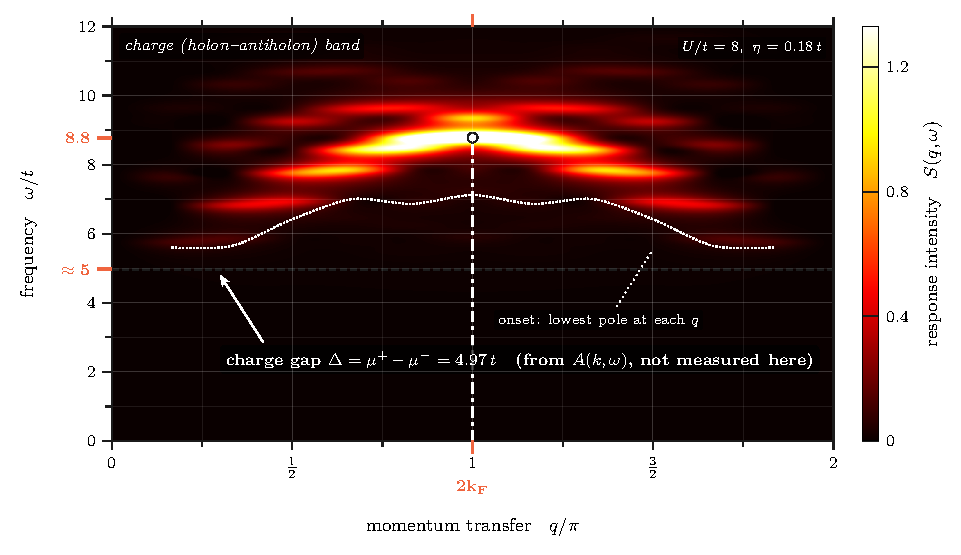
\includegraphics[width=0.92\textwidth]{figs/fig_sqw.pdf}
\caption{\textbf{Dynamical structure factor: the exact density response.} $S(q,\omega)$ of the
half-filled Hubbard chain ($U/t=8$, $L=12$, Lorentzian broadening $\eta=0.18\,t$)---the density--density
response, a number-conserving (neutral) excitation, computed exactly via the Haydock continued fraction
in the $N$-particle sector. Colour is the \emph{response intensity} $S(q,\omega)$ (units $1/t$): bright
means the system responds strongly at that $(q,\omega)$, dark means it does not. The weight forms the
two-particle charge (holon--antiholon) continuum, whose lower edge (dotted, the charge threshold)
sets the gap---as $q\to0$ it approaches $\Delta$---and traces the lower-boundary dispersion of the continuum; its diffuse upper boundary is left unmarked. Two features are decisive. \emph{(i)}
The continuum is \emph{gapped}: as $q\to0$ its lower edge approaches the charge gap
$\Delta=\mu^{+}-\mu^{-}=4.97\,t$ (exact $(N{\pm}1)$ ground-state energies)---the \emph{same} Mott gap that
separates the Hubbard bands in the single-particle channel (Fig.~\ref{fig:lattice}): two independent
dynamical observables, one correlation gap. \emph{(ii)} The continuum peaks at $q=2k_F=\pi$ at
$\omega\approx U\approx8\,t$, the bare Hubbard scale of a doubly-occupied site. The reflection
$S(q)=S(2\pi{-}q)$ holds to $\sim\!10^{-4}$ (Lanczos precision), and the analytic f-sum rule
$\int\omega\,S(q,\omega)\,d\omega\propto(1-\cos q)$ is recovered by the plotted (finite-window) grid to
$\sim\!0.3\%$. This is the collective observable the same bitstring-sampled primitive targets; as for
$A(k,\omega)$, faithfully sampling the \emph{full} response carries the sector-fraction cost of
Sec.~\ref{sec:resource}, where classically it needs a separate dynamical-DMRG computation.}\label{fig:sqw}\end{figure}

\begin{figure}[htbp]\centering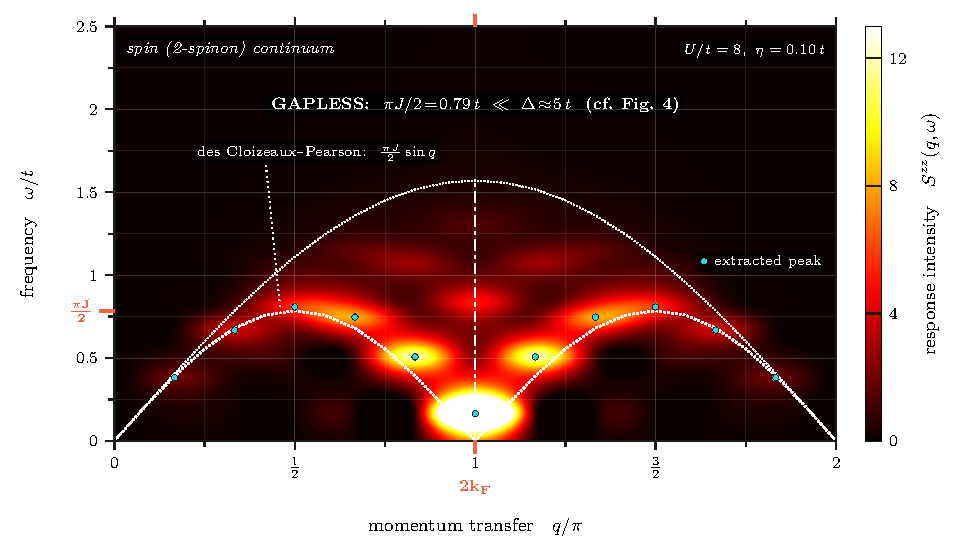
\includegraphics[width=0.92\textwidth]{figs/fig_spinqw.pdf}
\caption{\textbf{Spin structure factor: the gapless companion of the charge response.} The dynamical
spin structure factor $S^{zz}(q,\omega)$ of the same half-filled Hubbard chain ($U/t=8$, $L=12$; here
$\eta=0.10\,t$, finer because the spin scale is small), computed exactly by the Haydock continued fraction
from a spin seed $S^z_q\lvert\psi_0\rangle$ in the $N$-particle sector. \emph{Contrast Fig.~\ref{fig:sqw}}:
the charge response is \emph{gapped} by the Mott gap $\Delta\approx5\,t$, but the spin response is
\emph{gapless}---the two-spinon continuum touches $\omega=0$ at $q=0$ and $q=2k_F=\pi$. This is
spin--charge separation in the collective (two-particle) channel: charge and spin live in energetically
separate worlds, the spin set by the superexchange $J=4t^2/U=0.5\,t$, some $16\times$ smaller than $U$.
The spectral weight piles up on the des Cloizeaux--Pearson~\cite{descloizeaux1962} lower boundary $\tfrac{\pi J}{2}\lvert\sin q\rvert$
(dotted), bounded above by $\pi J\lvert\sin\tfrac q2\rvert$~\cite{mueller1981}; the numerically-extracted
peak dispersion (cyan markers) tracks this lower boundary to $\sim\!3\%$; the antiferromagnetic soft mode at $q=\pi$
carries the dominant weight. The reflection $S^{zz}(q)=S^{zz}(2\pi{-}q)$ holds to machine precision and
$S^{zz}(q{\to}0)\to0$ (total-$S^z$ conservation). The same bitstring-sampled primitive that yields
$A(k,\omega)$ and $S(q,\omega)$ targets this collective response as well.}\label{fig:spin}\end{figure}

\subsection{Fermionic magic marks the multireference regime}

Having validated the dynamical primitive, we now turn from the observable to its resource. The same
bitstring-sampled subspaces that reconstruct these spectra also let us evaluate, across the
nineteen-molecule suite, the one-body fermionic magic $\mathcal F_1=4\,\mathrm{tr}[\gamma(1-\gamma)]$
($=2N_{\mathrm u}$ for the closed-shell members) identified in Sec.~\ref{sec:resource}---and it
tracks precisely the \emph{multireference} character of the chemistry, not the sampling cost.

\begin{figure}[htbp]\centering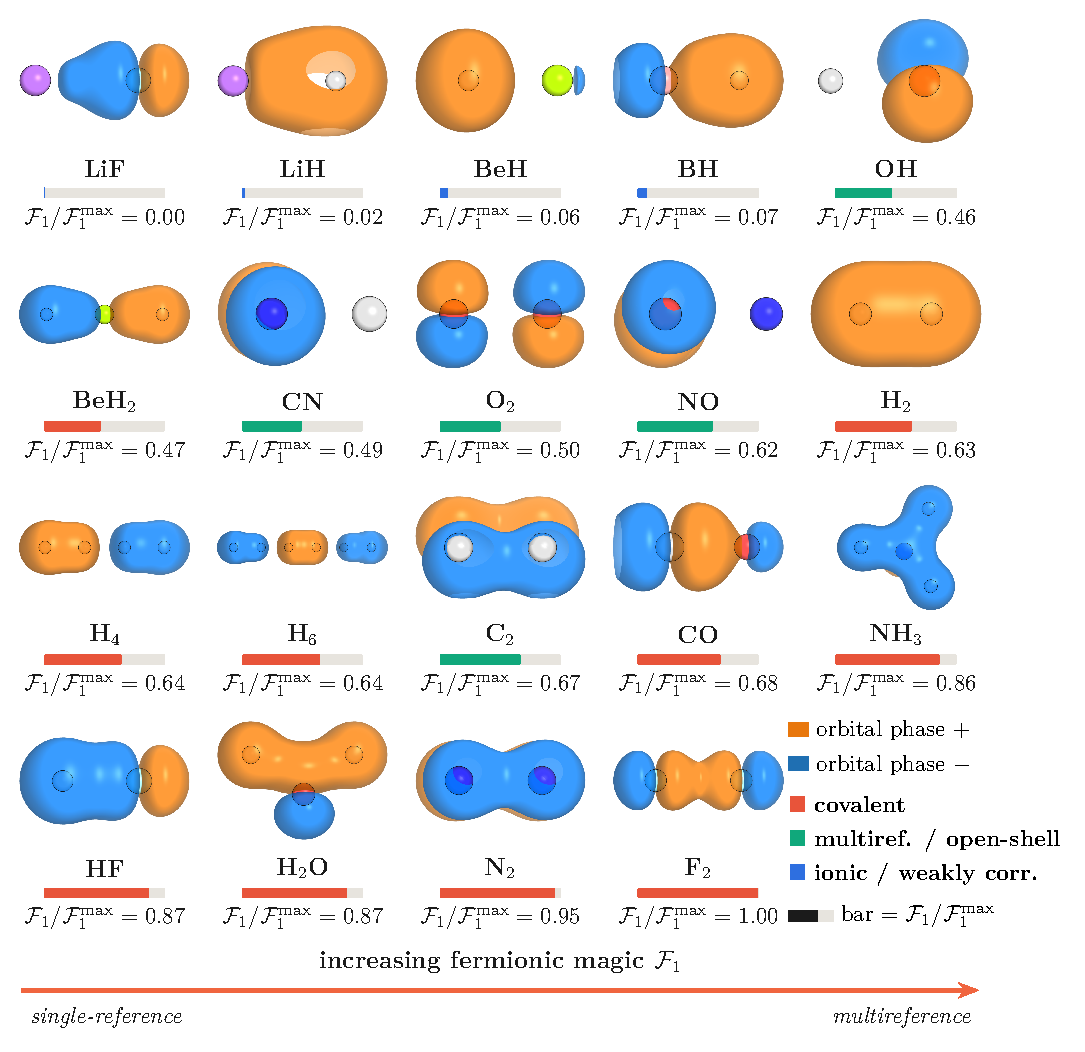
\includegraphics[width=\textwidth]{figs/fig_molecular_gallery.pdf}
\caption{\textbf{Nineteen molecules ordered by fermionic magic---the multireference axis.} The frontier
(HOMO) molecular orbital of each molecule at its dissociation geometry (PyMOL ray-traced two-phase
isosurface; orange/blue $=$ orbital phase $\pm$; CPK atoms), arranged left-to-right, top-to-bottom in
order of increasing FCI-verified fermionic magic (single-reference $\to$ strongly multireference). The
bar beneath each panel has length $\mathcal F_1/\mathcal F_1^{\max}$ and colour set by bonding regime; molecule names
are in neutral dark ink. The ordering makes the diagnostic visual: ionic and weakly-correlated bonds
(LiF, LiH, BeH, BH) sit at the near-Gaussian, single-reference end; covalent bond-breaking (HF,
$\mathrm{H_2O}$, $\mathrm{N_2}$, $\mathrm{F_2}$) at the strongly-multireference end; the inherently
multireference $\mathrm{C_2}$ and $\mathrm{O_2}$ in between. This one-body magic faithfully diagnoses
static-correlation character; it is decoupled from the sampling cost $|\mathcal S|$
(Sec.~\ref{sec:resource}, Fig.~\ref{fig:decoupling}). Orbitals are the mean-field frontier MO; the
magic ordering is the correlated, FCI-verified quantity.}\label{fig:gallery}\end{figure}

Across \textbf{nineteen molecules} spanning every bonding regime---covalent single, double, and triple
($\mathrm{H_2}$, $\mathrm{F_2}$, $\mathrm{C_2}$, $\mathrm{N_2}$, CO), polar and ionic (HF, LiF, LiH),
multi-centre ($\mathrm{H_2O}$, $\mathrm{NH_3}$, $\mathrm{BeH_2}$), metal hydrides (BH, BeH), open-shell
radicals (OH, CN, NO), the $\mathrm{O_2}$ triplet, and hydrogen chains ($\mathrm{H_4}$,
$\mathrm{H_6}$)---we compute the fermionic AntiFlatness in a valence bond-breaking active space,
\textbf{verifying every ground-state energy against exact active-space FCI to below $10^{-5}$~Ha}
(Figs.~\ref{fig:gallery},~\ref{fig:molsuite}, Table~\ref{tab:molecules}). On the same suite the sampling method reproduces
the exact (orbital-projected) spectral function $A(\omega)$ from bitstring-sampled subspaces to
relative-$L_1$ error below $10^{-3}$ at every molecule---at the dissociation geometry, using a sampled
subspace a fraction $\ge0.10$ of the $(N{+}1)$ sector, full only for the smallest ionic active spaces
where the sector itself is tiny (Table~\ref{tab:molecules})---so the
reconstruction is both exact and efficient across chemistry. The magic picture is sharp, and it is
\emph{not} a universal bond-length effect. Magic \emph{switches on} for covalent bond-breaking---rising from
near-Gaussian at equilibrium to a large fraction of its maximum on stretch ($\mathrm{F_2}$,
$\mathrm{N_2}$, $\mathrm{H_2O}$, HF, $\mathrm{NH_3}$, CO). It is \emph{already large at equilibrium} for
the inherently multireference $\mathrm{C_2}$ and $\mathrm{O_2}$, whose near-degenerate ground states
carry static correlation before any bond is stretched. And it \emph{stays near-Gaussian} for ionic and
weakly-correlated bonds (LiF, LiH, BH, BeH), whose dissociation remains essentially
single-configurational---the ionic--covalent avoided crossing of LiF lies well beyond the
stretch shown. Fermionic magic therefore tracks \emph{multireference, static-correlation} character,
not bond length \emph{per se}. This refines the qubit non-stabilizerness peak identified for molecular
bonding~\cite{sarkis2025} into a fermionic, Gaussian-referenced, FCI-verified statement: the fermionic
AntiFlatness~\cite{sierant2026,tarabunga2026}---efficiently computable from the Majorana covariance
matrix, and a genuine magic monotone for matchgate circuits~\cite{hebenstreit2019}---is a faithful
one-body diagnostic of static-correlation character, reading \emph{low} for the near-Gaussian LiF and
LiH and \emph{high} for stretched $\mathrm{N_2}$ or $\mathrm{F_2}$. As Sec.~\ref{sec:resource} makes
precise, this is a diagnostic of multireference character, not a predictor of the classical sampling
cost: the two are decoupled, and the cost of these strongly-correlated targets is set by the
higher-order structure the one-body magic does not resolve.

The $\mathrm{N_2}$ triple-bond dissociation ties the picture together (Fig.~\ref{fig:hero}): as the
bond stretches, the sharp quasiparticle feature of the addition spectrum $A(\omega)$ broadens into a
correlated multiplet and its integrated addition weight $\int A^{+}d\omega=1-\langle\hat n_p\rangle$
falls from $0.98$ to $0.52$ as the frontier orbital fills toward half-occupation on homolytic
dissociation. Along the same coordinate the fermionic magic rises as the \emph{exact} identity
$\mathcal F_1=2N_{\mathrm u}$ [Eq.~\eqref{eq:collapse}]---one-body magic \emph{is} the orbital-rotation-invariant
multireference count, the effective number of unpaired electrons $N_{\mathrm u}$ from the natural-orbital
occupations, which approaches its atomic limit of $6$---the two triplet $\mathrm{N}(^4S)$ atoms---as the
bond fully breaks ($N_{\mathrm u}\!=\!5.9$ at the largest stretch shown; $\mathcal F_1^{\rm diss}=11.38$, i.e.\
$N_{\mathrm u}=5.69$, at the finite dissociation geometry of Table~\ref{tab:molecules}). The
two curves in Fig.~\ref{fig:hero}(b)---the frontier-orbital addition weight and the static-correlation
magic---are distinct one-body diagnostics that cross as the bond breaks: the addition spectrum
redistributes from a single quasiparticle into a multiplet precisely as multireference character switches on. Fermionic magic is thus a computable, basis-independent proxy
for the strong static correlation that develops as the triple bond breaks.

\begin{figure}[htbp]\centering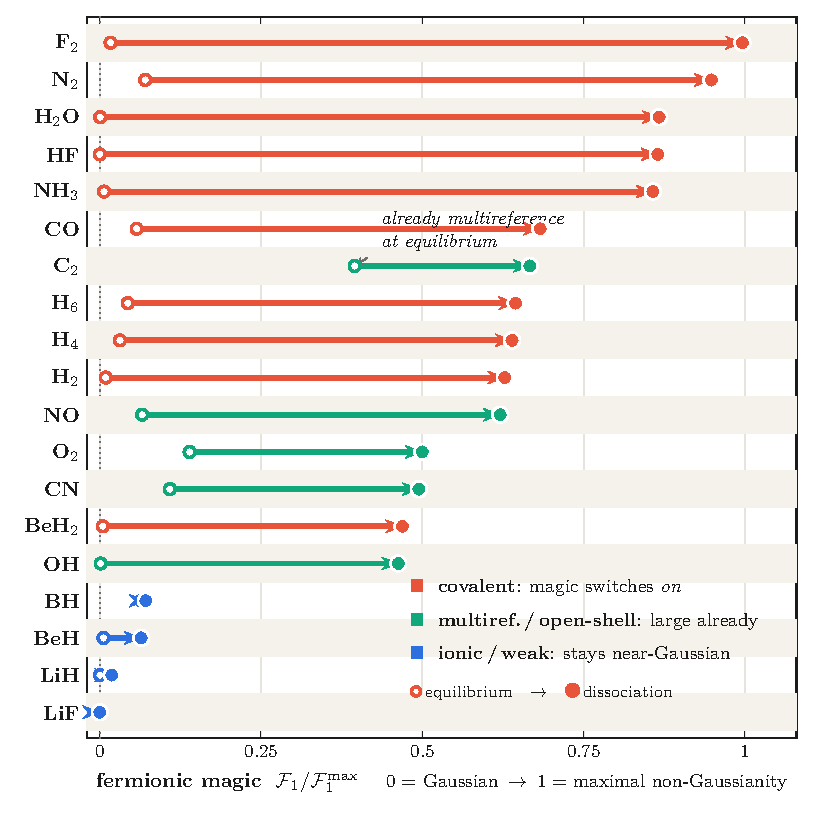
\includegraphics[width=0.9\textwidth]{figs/fig_molecular_suite.pdf}
\caption{\textbf{Fermionic magic marks the multireference regime across nineteen molecules.} Normalized
fermionic AntiFlatness $\mathcal F_1/\mathcal F_1^{\max}$ ($0$: Gaussian/mean-field; $1$: maximal non-Gaussianity) at
equilibrium (open circles) and at dissociation (filled), for all nineteen molecules, sorted by
dissociation magic and coloured by regime. Covalent bond-breaking switches magic on; the inherently
multireference $\mathrm{C_2}$ and $\mathrm{O_2}$ are already large at equilibrium; ionic and
weakly-correlated bonds (LiF, LiH, BH, BeH) stay near-Gaussian. Every ground-state energy is verified
against exact active-space FCI to $<10^{-5}$~Ha (Table~\ref{tab:molecules}); computed in valence
bond-breaking active spaces, cc-pVDZ.}\label{fig:molsuite}\end{figure}

\begin{figure}[htbp]\centering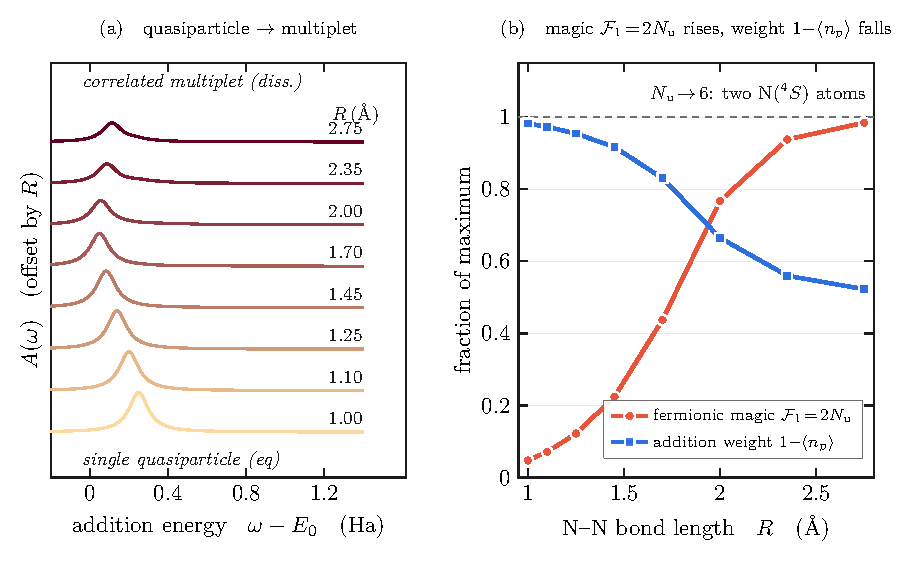
\includegraphics[width=\textwidth]{figs/fig_hero.pdf}
\caption{\textbf{Magic and multireference character in $\mathrm{N_2}$ dissociation.} (a)~The exact
addition spectral function $A(\omega)$ (orbital-projected, CAS(6,6), cc-pVDZ) along the triple-bond
stretch, offset by $R$: the sharp coherent quasiparticle peak at equilibrium ($R=1.0$~\AA) broadens
into a correlated multiplet on dissociation as its spectral weight collapses. (b)~Two physically
independent quantities along the same coordinate. The fermionic magic obeys the \emph{exact} identity
$\mathcal F_1=2N_{\mathrm u}$ [Eq.~\eqref{eq:collapse}, verified to $<10^{-13}$], so a single curve carries both: it rises
with the orbital-rotation-invariant multireference count---the effective number of unpaired electrons
$N_{\mathrm u}=\sum_i n_i(2-n_i)$ from the natural-orbital occupations $n_i$, approaching its atomic limit of $6$
(the two triplet $\mathrm{N}(^4S)$ atoms) as the bond fully breaks. The integrated addition weight $\int A^{+}d\omega=1-\langle\hat n_p\rangle$
(from panel a) falls from $0.98$ to $0.52$ over the same stretch; the two cross as the bond
breaks. Every geometry is FCI-verified to $<10^{-5}$~Ha.}\label{fig:hero}\end{figure}

\subsection{The time-evolution selector versus classical Krylov and CIPSI selectors}
The relevant question is not whether the sampled reconstruction is accurate---it is---but whether the
time-evolution selector (the selection strategy a quantum device implements, evaluated here in classical
simulation) discovers the important configurations more efficiently than deterministic classical
selectors at fixed subspace size. Averaged over twelve independent sampling seeds, the time-evolution
selector holds no robust advantage over classical polynomial Krylov and a
configuration-interaction perturbation-theory (CIPSI~\cite{cipsi1973,garniron2019}) Green's-function selector at small subspaces but moves ahead of
both in the strong-coupling corner once the subspace exceeds
$\sim\!120$ determinants: at $U/t=12$, $|\mathcal S|=200$ it reaches relative-$L_1$
$0.042\pm0.004$ against $0.729$ for deterministic Krylov and $0.431$ for CIPSI---a
tenfold reduction (Fig.~\ref{fig:bench})---because deterministic Krylov plateaus, unable to resolve the
delocalized configurations the strong-$U$ response demands, whereas the time-evolution selector reaches low
error with fewer discovered configurations. The same picture holds against budget-limited real-time
adaptive-sampling configuration interaction~\cite{tdasci2024}. At small subspace size there is
\emph{no} robust advantage: the win is over these two deterministic selectors and is asymptotic in
subspace size and coupling, not a small-scale artifact. We make no claim against the strongest classical
selector: heat-bath configuration interaction remains competitive with sample-based selection at
accessible sizes~\cite{reinholdt2025,holmeshci2016,sharmashci2017}, consistent with our own companion
review~\cite{review}. What drives the separation is the determinant count itself: the number of
configurations over which the strong-$U$ response spreads---and, with it, the extended-matchgate
circuit extent~\cite{extraferm}---grows with the evolution time the processor runs, while the quantum
sampling stays polynomial in the target subspace size $|\mathcal S|$. The fermionic magic grows alongside but, as Sec.~\ref{sec:resource}
establishes, does not itself set this cost.

\begin{figure}[htbp]\centering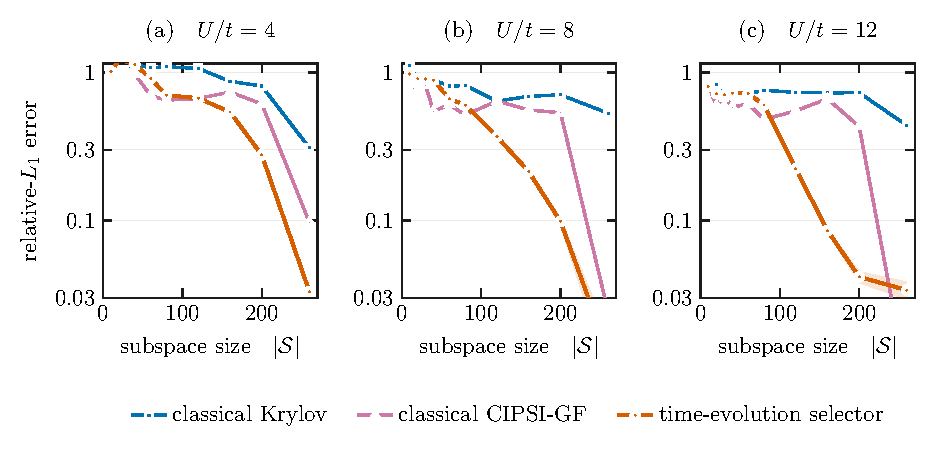
\includegraphics[width=0.97\textwidth]{figs/fig_benchmark.pdf}
\caption{\textbf{Time-evolution selector vs.\ classical Krylov and CIPSI selectors}, seed-averaged
(bands = seed spread; all curves evaluated in classical simulation). At strong coupling and
$|\mathcal S|\gtrsim120$ the time-evolution selector reaches low error with fewer discovered
configurations, while classical Krylov plateaus and the CIPSI perturbative Green's-function selector
trails; at small $|\mathcal S|$ there is no robust advantage.}\label{fig:bench}\end{figure}

\subsection{Scaling of the sampling cost with system size}
Across $L=4$--$14$ ($8$ to $28$ qubits---the three largest, $20$--$28$ qubits, reached by matrix-free
Lanczos/Haydock beyond the dense-diagonalization frontier and validated against it at $L\le8$; these
lattices are periodic rings, in contrast to the open chains of Sec.~\ref{sec:resource}) two
trends coexist (Fig.~\ref{fig:scaling}): the fermionic magic of the correlated ground state grows with
system size ($\mathcal F_1=6.6\to9.4\to12.8\to16.0\to19.3\to22.5$)---but only \emph{extensively}: per site
it is flat ($\mathcal F_1/L=1.65,1.56,1.60,1.60,1.61,1.61$), so a fixed amount of static correlation
accumulates with the sites and does not strengthen with size---while
the $(N{+}1)$-sector subspace \emph{fraction} needed to reconstruct $A(\omega)$ to relative-$L_1<0.05$
\emph{falls} steeply ($0.92\to0.82\to0.56\to0.36\to0.17\to0.08$, i.e.\ from $92\%$ to $8\%$), the favourable
face of the polynomial-shot bound of Theorem~\ref{thm:b2} (App.~\ref{app:b2}) and consistent with the
convergence behaviour established for sample-based Krylov
diagonalization~\cite{skqd2025,yoshioka2025}. The absolute subspace $|\mathcal S|$ nonetheless grows---
indeed, for these lattice models it grows \emph{exponentially} with system size, an intrinsic
consequence of the computational-basis delocalization of the ground state~\cite{gaberle2026}. Quantitatively,
a least-squares fit over $L=4$--$14$ gives $|\mathcal S|\sim e^{1.05\,L}$ ($R^2=0.998$)---exponential, but
\emph{slower} than the full $(N{+}1)$ sector $D\sim e^{1.30\,L}$, so the required fraction contracts as
$\sim e^{-0.25\,L}$ (halving every $\sim2.8$ sites, $R^2=0.94$). Figure~\ref{fig:scaling}
is therefore not a claim of small \emph{absolute} cost but the complementary, quantitative statement that the
\emph{fraction} of the sector required for a fixed spectral accuracy shrinks exponentially. And what tracks that
absolute size is not the magic but the entanglement, as a direct chain-versus-ladder test makes concrete
(Fig.~\ref{fig:ladder}). At \emph{matched} one-body magic---a two-leg Hubbard ladder~\cite{nogaki2025} and
a chain of the same site count have near-identical $\mathcal F_1$ ($12.82$ vs $12.91$ at $16$ qubits, half
filling, $U/t=8$), since $\mathcal F_1$ is a geometry-blind one-body invariant---the ladder's
perpendicular cut carries an area-law boundary of two legs rather than one, so its minimal bond dimension
is far larger ($\chi=8\to38$ at $16$ qubits; the chain-to-ladder ratio reads $\times2.6$, $\times4.8$, $\times6.3$
at $12$, $16$ and $20$ qubits, the ladder $\chi$ saturating at $38$ while the chain $\chi$ is non-monotone ($5,8,6$), so the last step arises from the chain falling $8\to6$ rather than from ladder growth) and its response-targeted $(N{\pm}1)$ fraction correspondingly higher
($0.43\to0.63$). The cost is lower-bounded and tracked by the bond dimension $\chi$, not by $\mathcal F_1$---the
decoupling of Sec.~\ref{sec:resource}, now exhibited as a controlled contrast in which the classical cost
tracks $\chi$ and not $\mathcal F_1$. We are explicit about scope: a two-leg ladder with
$\chi\!\approx\!38$ is quasi-one-dimensional and remains near-exact for (dynamical) density-matrix
renormalization group~\cite{paeckel2019,jeckelmann2002}---it is \emph{not} itself beyond the tensor-network
frontier, which lies in genuinely two-dimensional (wide-cylinder) geometries and the all-to-all orbital
graphs of quantum chemistry. What the ladder isolates is the \emph{resource} statement---that entanglement,
not one-body magic, lower-bounds and tracks the determinant support. Because $\chi$ is precisely the bond dimension a
(dynamical) density-matrix renormalization-group calculation must carry~\cite{paeckel2019,jeckelmann2002},
panel~(a) is a direct classical-cost comparison: the $\times4.8$ chain-to-ladder gap at fixed
$\mathcal F_1$ ($16$ qubits) is a gap in the tensor-network spectral cost itself, and by Prop.~\ref{prop:chibound}
it is a rigorous lower bound on the raw determinant support---a resource contrast, with no
beyond-classical claim asserted.

\begin{figure}[htbp]\centering% self-contained native pgfplots fragment (fig:scaling) -- DATA-DRIVEN from scaling_data.json
% (real Lanczos/Haydock scaling data, L=4,6,8,10,12,14; U=8).
% Panel (c) added 2026-08-17: absolute support |S|=frac*Np1_sector and sector dim D=Np1_sector vs 2L
% (Np1_sector=[24,300,3920,52920,731808,10306296]; both grow exponentially, D faster than |S|).
\definecolor{scMag}{HTML}{D55E00}\definecolor{scFrac}{HTML}{0072B2}\definecolor{scInk}{HTML}{5B5B5B}
\definecolor{inkPrim}{HTML}{1B1B1B}\definecolor{scDim}{HTML}{8A8A8A}
\begin{tikzpicture}
\begin{groupplot}[group style={group size=3 by 1, horizontal sep=0.95cm},
  width=5.0cm, height=5.5cm, paperaxis,
  xmin=6.5, xmax=29.5, xtick={8,16,24}, xtick align=outside,
  title style={at={(0,1)},anchor=south west,font=\small\bfseries,yshift=1.5pt},
  label style={font=\small}, tick label style={font=\footnotesize},
  every node near coord/.append style={font=\scriptsize,inkPrim,anchor=south,yshift=1pt}]
% ---------- (a) fermionic magic grows ----------
\nextgroupplot[title={(a)~magic grows},
  xlabel={qubits $\;2L$}, ylabel={fermionic magic $\mathcal{F}_1$}, ymin=0, ymax=30.5,
  ytick={0,10,20,30}, ymajorgrids, grid style={draw=black!10}]
\addplot[draw=none,fill=scMag,fill opacity=0.10] coordinates {(8,6.6074) (12,9.3851) (16,12.8138) (20,16.0183) (24,19.2721) (28,22.5050)} \closedcycle;
\addplot[scMag,line width=1.3pt,mark=*,mark size=2.5pt,mark options={fill=scMag,draw=white,line width=0.7pt},
  nodes near coords,point meta=explicit symbolic]
  coordinates {(8,6.6074)[6.6] (12,9.3851)[] (16,12.8138)[] (20,16.0183)[] (24,19.2721)[] (28,22.5050)[22.5]};
% ---------- (b) subspace fraction falls ----------
\nextgroupplot[title={(b)~fraction falls},
  xlabel={qubits $\;2L$}, ylabel={$|\mathcal{S}|/\dim$}, ymin=0, ymax=1.08,
  ytick={0,0.5,1}, ymajorgrids, grid style={draw=black!10}]
\fill[scFrac,fill opacity=0.05] (axis cs:6.5,0) rectangle (axis cs:29.5,0.5);
\node[inkPrim,font=\footnotesize\itshape,anchor=west] at (axis cs:7.2,0.19) {beyond-classical};
\addplot[draw=none,fill=scFrac,fill opacity=0.10] coordinates {(8,0.9167) (12,0.8200) (16,0.5561) (20,0.3625) (24,0.1700) (28,0.0800)} \closedcycle;
\addplot[scFrac,line width=1.3pt,mark=square*,mark size=2.4pt,mark options={fill=scFrac,draw=white,line width=0.7pt},
  nodes near coords,point meta=explicit symbolic]
  coordinates {(8,0.9167)[0.92] (12,0.8200)[] (16,0.5561)[] (20,0.3625)[] (24,0.1700)[] (28,0.0800)[0.08]};
% ---------- (c) absolute size grows exponentially ----------
\nextgroupplot[title={(c)~absolute size grows},
  xlabel={qubits $\;2L$}, ylabel={count}, ymode=log, ymin=8, ymax=8e7,
  ytick={1e1,1e3,1e5,1e7}, ymajorgrids, grid style={draw=black!10},
  legend style={font=\scriptsize,at={(0.03,0.98)},anchor=north west,draw=none,fill=white,fill opacity=0.55,text opacity=1,row sep=0.4pt,inner sep=1.5pt},legend cell align=left]
\addplot[scDim,line width=1.3pt,mark=triangle*,mark size=2.6pt,mark options={fill=scDim,draw=white,line width=0.6pt}]
  coordinates {(8,24) (12,300) (16,3920) (20,52920) (24,731808) (28,10306296)};
\addlegendentry{sector $\dim$ $\sim e^{1.30L}$}
\addplot[scFrac,line width=1.3pt,mark=square*,mark size=2.3pt,mark options={fill=scFrac,draw=white,line width=0.6pt}]
  coordinates {(8,22) (12,246) (16,2180) (20,19184) (24,124407) (28,824504)};
\addlegendentry{support $|\mathcal S|$ $\sim e^{1.05L}$}
\end{groupplot}
\end{tikzpicture}

\caption{\textbf{Scaling of the sampling cost with system size} ($L=4$--$14$; 8--28 qubits, half-filled
\emph{periodic} Hubbard rings at $U/t=8$; the three largest sizes ($20$--$28$ qubits) computed by matrix-free
Lanczos/Haydock, validated against dense diagonalization at $L\le8$). (a)~The fermionic magic $\mathcal F_1$ of the
correlated ground state grows with system size ($6.6\to22.5$), extensively---$\mathcal F_1/L$ is flat at
$\approx\!1.6$, so this is accumulation, not strengthening, of static correlation. (b)~The $(N{+}1)$-sector subspace fraction
$|\mathcal S|/\dim$ needed to reconstruct $A(\omega)$ to relative-$L_1<0.05$ \emph{falls} steeply
($0.92\to0.08$)---the sampled reconstruction becomes relatively cheaper as the state grows
harder to represent classically. \textbf{(c)}~The absolute sizes nonetheless both grow
\emph{exponentially} (log scale): the determinant support $|\mathcal S|\sim e^{1.05\,L}$ and the full
$(N{+}1)$ sector dimension $\dim\sim e^{1.30\,L}$; the faster-growing sector is precisely why the
\emph{fraction} in (b) contracts. Fraction down, absolute cost up---the honest two-sided
picture.}\label{fig:scaling}\end{figure}

\begin{figure}[htbp]\centering% G1 (landmark): chain vs 2-leg ladder at MATCHED one-body magic F1 -- exact ED (ladder_vs_chain.json).
% At matched F1 the ladder's minimal bond dimension chi and required (N+-1) fraction diverge from the
% chain's: the cost is governed by entanglement (chi), not F1 -- a controlled resource contrast
% (a width-38 ladder is still classically near-exact for DMRG; no beyond-classical claim).
\definecolor{ldChain}{HTML}{0072B2}\definecolor{ldLad}{HTML}{D55E00}\definecolor{ldInk}{HTML}{1B1B1B}
\begin{tikzpicture}
\begin{groupplot}[group style={group size=2 by 1, horizontal sep=1.9cm},
  width=8.0cm, height=6.0cm, paperaxis,
  xmin=10.5, xmax=21.5, xtick={12,16,20}, xtick align=outside,
  title style={at={(0,1)},anchor=south west,font=\normalsize\bfseries,yshift=2pt},
  label style={font=\normalsize}, tick label style={font=\normalsize},
  legend style={font=\footnotesize,draw=black!25,fill=white,fill opacity=0.9,text opacity=1},legend cell align=left]
% ---------- (a) minimal bond dimension chi ----------
\nextgroupplot[title={(a)~minimal bond dimension $\chi$},
  xlabel={qubits $\;2L$}, ylabel={$\chi$ (min.\ MPS bond dim.)}, ymin=0, ymax=48,
  ytick={0,10,20,30,40}, ymajorgrids, grid style={draw=black!10},
  legend pos=north west]
\addplot[ldLad,line width=1.5pt,mark=*,mark size=3pt,mark options={fill=ldLad,draw=white,line width=0.8pt}]
  coordinates {(12,13)(16,38)(20,38)}; \addlegendentry{2-leg ladder}
\addplot[ldChain,line width=1.5pt,mark=square*,mark size=2.8pt,mark options={fill=ldChain,draw=white,line width=0.8pt}]
  coordinates {(12,5)(16,8)(20,6)}; \addlegendentry{chain}
\node[ldInk,font=\scriptsize,anchor=north east] at (axis cs:21.3,46.5) {$\mathcal F_1$ matched};
\node[ldInk,font=\scriptsize,anchor=south] at (axis cs:16,41.0) {$\times4.8$};
% ---------- (b) required (N+-1) fraction ----------
\nextgroupplot[title={(b)~sampled $(N{\pm}1)$ fraction},
  xlabel={qubits $\;2L$}, ylabel={$|\mathcal S|/D$ for rel-$L_1<0.05$}, ymin=0, ymax=1.0,
  xmin=10.5, xmax=17.5, xtick={12,16}, ytick={0,0.25,0.5,0.75,1}, ymajorgrids, grid style={draw=black!10},
  legend pos=south west]
\addplot[ldLad,line width=1.5pt,mark=*,mark size=3pt,mark options={fill=ldLad,draw=white,line width=0.8pt}]
  coordinates {(12,0.807)(16,0.626)}; \addlegendentry{2-leg ladder}
\addplot[ldChain,line width=1.5pt,mark=square*,mark size=2.8pt,mark options={fill=ldChain,draw=white,line width=0.8pt}]
  coordinates {(12,0.717)(16,0.426)}; \addlegendentry{chain}
\node[ldInk,font=\scriptsize,anchor=north east] at (axis cs:17.3,0.97) {same $\mathcal F_1$};
\end{groupplot}
\end{tikzpicture}

\caption{\textbf{The cost is tracked by entanglement, not one-body magic---a controlled chain-versus-ladder
contrast.} A two-leg Hubbard ladder versus a chain of the \emph{same} site count (half filling,
$U/t=8$; exact diagonalization). At matched fermionic magic $\mathcal F_1$ (open chain vs.\ ladder: $9.60/9.69$,
$12.82/12.91$, $16.03/16.09$ at $12/16/20$ qubits---$\mathcal F_1$ is a geometry-blind one-body invariant)
the ladder's perpendicular cut has an area-law boundary of two rather than one. \textbf{(a)}~Its minimal
matrix-product-state bond dimension $\chi$ is far larger; the chain-to-ladder ratio grows over
$12\to20$ qubits ($\times2.6,\times4.8,\times6.3$), the ladder $\chi$ saturating at $38$ while the chain
$\chi$ stays small and does \emph{not} grow ($5,8,6$ at $12/16/20$ qubits---non-monotone, with no systematic
increase over this range, consistent with the at most logarithmic entanglement growth of the gapless spin
sector)---the reported $\chi$ are threshold-truncated Schmidt ranks. \textbf{(b)}~The response-targeted $(N{\pm}1)$ fraction needed for spectral
relative-$L_1<0.05$ is correspondingly higher for the ladder (these union $(N{\pm}1)$ response fractions
differ from the single-sector $(N{+}1)$ $A(\omega)$ fractions of Fig.~\ref{fig:scaling}, a different
observable). Same one-body magic, higher cost: the
determinant support is lower-bounded and tracked by the basis-dependent bond dimension $\chi$ (Sec.~\ref{sec:resource}), not
by $\mathcal F_1$. A ladder of this width ($\chi\!\approx\!38$) remains classically near-exact for dynamical
DMRG; it is a resource contrast, not a beyond-classical claim.}\label{fig:ladder}\end{figure}
